\documentclass[12pt]{article}
\usepackage{hyperref}
\usepackage{listings}
\usepackage{biblatex}
\usepackage{tikz}
\usepackage{refstyle}
\usepackage{mathabx}
\usepackage{amssymb}
\usepackage{caption}
\usepackage{float}
\usepackage{graphicx}
\usepackage{graphics}
\usepackage{subfig}

\graphicspath{{/storage/self/primary/Download/latexnew/fig}}
\begin{document}
\title{\textbf{PLATFORMIO}}
\date{}
\maketitle
\begin{enumerate}
    \item \textbf{Question(GATE-IN-2021-36):}Given below \figref{fig:1} is the diagram of a synchronous sequential circuit with one $J-K$ flip-flop and one $T$ flip-flop with their outputs denoted as A and B respectively,with$J_A = (A'+B'),K_A = (A+B)$,and $T_B = A.$


\begin{figure}[H]
        \centering
	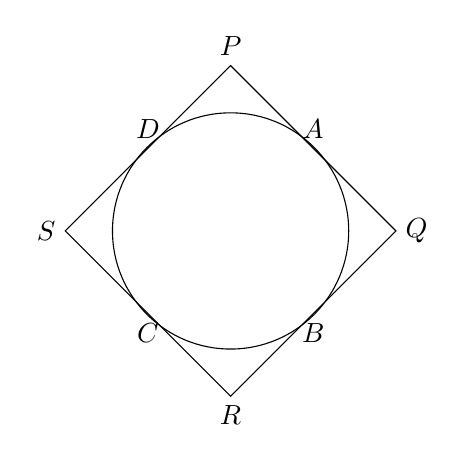
\begin{tikzpicture}
     \draw (0,0)circle(1.5cm);    
     \draw (-2.1,0)-- node[below]{$C$}(0,-2.1)--node[below]{$B$}(2.1,0)--node[above]{$A$}(0,2.1)--node[above]{$D$}cycle;
     \node[right] at (2.1,0){$Q$};    
     \node[left] at (-2.1,0){$S$};
     \node[above] at (0,2.1){$P$};
     \node[below] at (0,-2.1){$R$};    
\end{tikzpicture}

        \caption{}
        \label{fig:fig:1}
\end{figure}

   
    Starting from the initial state $(AB=00)$,the sequence of states $(AB)$ visited by the circuit is
    \begin{enumerate}
	    \item $00\rightarrow01\rightarrow10\rightarrow11\rightarrow00 ...$
        \item $00\rightarrow10\rightarrow01\rightarrow11\rightarrow00 ...$
        \item $00\rightarrow10\rightarrow11\rightarrow01\rightarrow00 ...$
        \item $00\rightarrow01\rightarrow11\rightarrow00 ...$
    \end{enumerate}


\end{enumerate}


\end{document}
